% Generated from reviewed lane; compile via book/textbook.tex.
\clearpage

原书 PDF 页 76；印刷页码 63。

\href{source-images/pdf-076.jpeg}{查看原页}

即 \(\{U_n(x)\}\) 是区间 \([-1,1]\) 上带权 \(\rho(x)=\sqrt{1-x^2}\) 的正交多项式族。还可得到递推关系式

\[
U_0(x)=1,\quad U_1(x)=2x,
\]

\[
U_{n+1}(x)=2xU_n(x)-U_{n-1}(x)\quad(n=1,2,\cdots).
\]

\paragraph{2. Laguerre 多项式}\label{ch03b-laguerre-ux591aux9879ux5f0f}

在区间 \([0,\infty)\) 上带权 \(\rho(x)=\mathrm e^{-x}\) 的正交多项式称为 Laguerre 多项式，其表达式为

\[
L_n(x)=\mathrm e^n\frac{\mathrm d^n}{\mathrm dx^n}(x^n\mathrm e^{-x}).\tag{3.4.11}
\]

它也具有正交性质

\[
\int_0^\infty \mathrm e^{-x}L_n(x)L_m(x)\,\mathrm dx=
\begin{cases}
0,&m\ne n,\\
(n!)^2,&m=n
\end{cases}
\]

和递推关系

\[
L_0(x)=1,\quad L_1(x)=1-x,
\]

\[
L_{n+1}(x)=(1+2n-x)L_n(x)-n^2L_{n-1}(x)\quad(n=1,2,\cdots).
\]

\paragraph{3. Hermite 多项式}\label{ch03b-hermite-ux591aux9879ux5f0f}

在区间 \((-\infty,\infty)\) 上带权 \(\rho(x)=\mathrm e^{-x^2}\) 的正交多项式称为 Hermite 多项式，其表达式为

\[
H_n(x)=(-1)^n\mathrm e^{x^2}\frac{\mathrm d^n}{\mathrm dx^n}(\mathrm e^{-x^2}).\tag{3.4.12}
\]

它满足正交关系

\[
\int_{-\infty}^{+\infty}\mathrm e^{-x^2}H_m(x)H_n(x)\,\mathrm dx=
\begin{cases}
0,&m\ne n,\\
2^nn!\sqrt\pi,&m=n,
\end{cases}
\]

并有递推关系

\[
H_0(x)=1,\quad H_1(x)=2x,
\]

\[
H_{n+1}(x)=2xH_n(x)-2nH_{n-1}(x)\quad(n=1,2,\cdots).
\]

\subsection{3.5 函数按正交多项式展开}\label{ch03b-ux51fdux6570ux6309ux6b63ux4ea4ux591aux9879ux5f0fux5c55ux5f00}

设 \(f(x)\in C[a,b]\)，用正交多项式 \(\{g_0(x),g_1(x),\cdots,g_n(x)\}\) 作基，求最佳平方逼近多项式

\[
S_n(x)=a_0g_0(x)+a_1g_1(x)+\cdots+a_ng_n(x).\tag{3.5.1}
\]

由 \(\{g_k(x)\}\) 的正交性及式 (3.3.13)，可求得系数

\[
a_k=\frac{(f,g_k)}{(g_k,g_k)}\quad(k=0,1,\cdots,n),\tag{3.5.2}
\]

于是，\(f(x)\) 的最佳平方逼近多项式为

\begin{quote}
校注（agent 补充）：式 (3.4.11) 的原扫描明确印为 \(\mathrm e^n\)，已忠实保留；这是疑似原书错误，不是 OCR 误读。取 \(n=0\)，原式给出 \(L_0(x)=\mathrm e^{-x}\)，与紧接着印出的 \(L_0(x)=1\) 矛盾。相容的 Rodrigues 表达式前因子应为 \(\mathrm e^x\)。见 \href{verified/assets/ch03b/p076-laguerre-formula.png}{原式放大裁切}。
\end{quote}

\clearpage

原书 PDF 页 77；印刷页码 64。

\href{source-images/pdf-077.jpeg}{查看原页}

\[
S_n(x)=\sum_{k=0}^n\frac{(f,g_k)}{(g_k,g_k)}g_k(x).\tag{3.5.3}
\]

由式 (3.3.15) 可得均方误差为

\[
\|\delta_n\|_2=\|f-S_n\|_2=\sqrt{\|f\|_2^2-\sum_{k=0}^n\frac{(f,g_k)}{(g_k,g_k)}(f,g_k)}.\tag{3.5.4}
\]

若 \(f(x)\) 在 \([a,b]\) 上按正交多项式 \(\{g_k(x)\}\) 展开，系数 \(a_k\)（\(k=0,1,\cdots\)）按式 (3.5.2) 计算，这样可得到 \(f(x)\) 的展开式

\[
f(x)\sim\sum_{k=0}^\infty a_kg_k(x).\tag{3.5.5}
\]

式 (3.5.5) 右端级数称为广义 Fourier 级数，系数 \(a_k\) 称为广义 Fourier 系数，它是 Fourier 级数的直接推广。从以上讨论可知，任何 \(f(x)\in C[a,b]\) 均可展开成广义 Fourier 级数，其部分和 \(S_n(x)\) 是 \(f(x)\) 的最佳平方逼近，系数 \(a_k\) 与 \(n\) 无关，因此，当 \(n\) 增加时，只要多计算增加的系数 \(a_k\)。级数 (3.5.5) 可能不一致收敛于 \(f(x)\)，但在 \(f(x)\) 满足一定条件下也可一致收敛到 \(f(x)\)。

下面考虑函数 \(f(x)\in C[-1,1]\) 按 Legendre 多项式 \(\{P_0(x),P_1(x),\cdots\}\) 展开的最佳平方逼近多项式 \(S_n^*(x)\)。由式 (3.5.1) 和式 (3.5.2) 可得

\[
S_n^*(x)=a_0^*P_0(x)+a_1^*P_1(x)+\cdots+a_n^*P_n(x),\tag{3.5.6}
\]

其中

\[
a_k^*=\frac{(f,P_k)}{(P_k,P_k)}=\frac{2k+1}{2}\int_{-1}^1f(x)P_k(x)\,\mathrm dx.\tag{3.5.7}
\]

根据式 (3.5.4)，平方误差为

\[
\|\delta_k\|_2^2=\int_{-1}^1 f^2(x)\,\mathrm dx-\sum_{k=0}^n\frac{2}{2k+1}(a_k^*)^2.\tag{3.5.8}
\]

\textbf{例 3.4} 求 \(f(x)=\mathrm e^x\) 在 \([-1,1]\) 上的三次最佳平方逼近多项式。

\textbf{解} 先计算 \((f,P_k)\)（\(k=0,1,2,3\)），即

\[
(f,P_0)=\int_{-1}^1\mathrm e^x\,\mathrm dx=\mathrm e-\frac1{\mathrm e}\approx2.3504,
\]

\[
(f,P_1)=\int_{-1}^1x\mathrm e^x\,\mathrm dx=2\mathrm e^{-1}\approx0.7358,
\]

\[
(f,P_2)=\int_{-1}^1\left(\frac32x^2-\frac12\right)\mathrm e^x\,\mathrm dx=\mathrm e-\frac7{\mathrm e}\approx0.1431,
\]

\[
(f,P_3)=\int_{-1}^1\left(\frac52x^3-\frac32x\right)\mathrm e^x\,\mathrm dx=37\frac1{\mathrm e}-5\mathrm e\approx0.02013.
\]

由式 (3.5.7) 得

\[
a_0^*=(f,P_0)/2=1.1752,\quad a_1^*=3(f,P_1)/2=1.1036,
\]

\[
a_2^*=5(f,P_2)/2=0.3578,\quad a_3^*=7(f,P_3)/2=0.07046,
\]

代入式 (3.5.6)，得

\begin{quote}
校注（agent 补充）：式 (3.5.8) 左端原书印为 \(\|\delta_k\|_2^2\)，已保留。其右端求和上限为 \(n\)，与前式 (3.5.4) 一致时左端应记为 \(\|\delta_n\|_2^2\)，属疑似原书下标错误。见 \href{verified/assets/ch03b/p077-error-formula.png}{原式放大裁切}。
\end{quote}

\clearpage

原书 PDF 页 78；印刷页码 65。

\href{source-images/pdf-078.jpeg}{查看原页}

\[
S_3^*(x)=0.9963+0.9979x+0.5367x^2+0.1761x^3.
\]

均方误差为

\[
\|\delta_n\|_2=\|\mathrm e^x-S_3^*(x)\|_2=\sqrt{\int_{-1}^1\mathrm e^{2x}\,\mathrm dx-\sum_{k=0}^3\frac{2}{2k+1}(a_k^*)^2}\leqslant0.0084,
\]

最大误差为

\[
\|\delta_n\|_\infty=\|\mathrm e^x-S_3(x)\|_\infty\leqslant0.0112.
\]

如果 \(f(x)\in C[a,b]\)，求 \(f(x)\) 在区间 \([a,b]\) 上的最佳平方逼近多项式。作变换

\[
x=\frac{b-a}{2}t+\frac{b+a}{2}\quad(-1\leqslant t\leqslant1),
\]

于是

\[
F(t)=f\left(\frac{b-a}{2}t+\frac{b+a}{2}\right).
\]

在 \([-1,1]\) 上可用 Legendre 多项式作最佳平方逼近多项式 \(S_n^*(t)\)，从而得到 \(f(x)\) 在区间 \([a,b]\) 上的最佳平方逼近多项式 \(S_n^*\left(\dfrac1{b-a}(2x-a-b)\right)\)。

由于 Legendre 多项式 \(\{P_k(x)\}\) 是在区间 \([-1,1]\) 上由 \(\{1,x,x^2,\cdots,x^k,\cdots\}\) 正交化得到的，因此利用函数的 Legendre 展开部分和得到最佳平方逼近多项式与由

\[
S^*(x)=a_0+a_1x+\cdots+a_nx^n
\]

直接通过解法方程得到的 \(H_n\) 中的最佳平方逼近多项式是一致的，只是当 \(n\) 较大时求法方程会出现病态方程，计算误差较大，不能使用。而用 Legendre 展开不用解线性方程组，不存在病态问题，计算公式使用起来也较方便，因此通常都用此法求最佳平方逼近多项式。

\subsection{3.6 曲线拟合的最小二乘法}\label{ch03b-ux66f2ux7ebfux62dfux5408ux7684ux6700ux5c0fux4e8cux4e58ux6cd5}

\subsubsection{3.6.1 一般的最小二乘逼近}\label{ch03b-ux4e00ux822cux7684ux6700ux5c0fux4e8cux4e58ux903cux8fd1}

在科学实验的统计方法研究中，往往要从一组实验数据 \((x_i,y_i)\)（\(i=0,1,\cdots,m\)）中寻找自变量 \(x\) 与因变量 \(y\) 之间的函数关系 \(y=F(x)\)。由于观测数据往往不准确，因此不要求 \(y=F(x)\) 经过所有点 \((x_i,y_i)\)，而只要求在给定点 \(x_i\) 上误差 \(\delta_i=F(x_i)-y_i\)（\(i=0,1,\cdots,m\)）按某种标准最小。若记 \(\boldsymbol\delta=(\delta_0,\delta_1,\cdots,\delta_m)^{\mathrm T}\)，就是要求向量 \(\boldsymbol\delta\) 的范数 \(\|\boldsymbol\delta\|\) 最小。如果用最大范数，计算上困难较大，通常就采用 Euclid 范数 \(\|\boldsymbol\delta\|_2\) 作为误差度量的标准。关于最小二乘法的一般提法是：对于给定的一组数据 \((x_i,y_i)\)（\(i=0,1,\cdots,m\)），要求在函数空间 \(\Phi=\operatorname{span}\{\varphi_0,\varphi_1,\cdots,\varphi_n\}\) 中找一个函数 \(y=S^*(x)\)，使误差平方和

\begin{quote}
校注（agent 补充）：本页最大误差式原书写 \(S_3(x)\)，而同例的最佳平方逼近多项式记作 \(S_3^*(x)\)；转录保留原来的无星号记法。
\end{quote}

\clearpage

原书 PDF 页 79；印刷页码 66。

\href{source-images/pdf-079.jpeg}{查看原页}

\[
\|\boldsymbol\delta\|_2^2=\sum_{i=0}^m\delta_i^2=\sum_{i=0}^m[S^*(x_i)-y_i]^2=\min_{S(x)\in\varphi}\sum_{i=1}^m[S(x_i)-y_i]^2,\tag{3.6.1}
\]

这里

\[
S(x)=a_0\varphi_0(x)+a_1\varphi_1(x)+\cdots+a_n\varphi_n(x)\quad(n<m).\tag{3.6.2}
\]

这就是一般的最小二乘逼近，用几何语言说，就称为曲线拟合的最小二乘法。

用最小二乘法求拟合曲线时，首先要确定 \(S(x)\) 的形式。这不是单纯数学问题，还与所研究问题的运动规律及所得观测数据 \((x_i,y_i)\) 有关；通常要从问题的运动规律及给定数据描图来确定 \(S(x_i)\) 的形式，并通过实际计算选出较好的结果------这点将从下面的例题得到说明。\(S(x)\) 的一般表达式为式 (3.6.2) 所示的线性形式。若 \(\varphi_k(x)\) 是 \(k\) 次多项式，\(S(x)\) 就是 \(n\) 次多项式。为了使问题的提法更有一般性，通常把最小二乘法中 \(\|\boldsymbol\delta\|_2^2\) 都考虑为加权平方和

\[
\|\boldsymbol\delta\|_2^2=\sum_{i=0}^m\omega(x_i)[S(x_i)-f(x_i)]^2.\tag{3.6.3}
\]

这里 \(\omega(x)\geqslant0\) 是 \([a,b]\) 上的权函数，它表示不同点 \((x_i,f(x_i))\) 处的数据比重不同，例如，\(\omega(x_i)\) 可表示在点 \((x_i,f(x_i))\) 处重复观测的次数。用最小二乘法求拟合曲线的问题，就是在形如式 (3.6.2) 的 \(S(x)\) 中求一函数 \(y=S^*(x)\)，使式 (3.6.3) 取得最小。它转化为求多元函数

\[
I(a_0,a_1,\cdots,a_n)=\sum_{i=0}^m\omega(x_i)\left[\sum_{j=0}^na_j\varphi_j(x_i)-f(x_i)\right]^2\tag{3.6.4}
\]

的极小点 \((a_0^*,a_1^*,\cdots,a_n^*)\) 问题。这与 3.3 节讨论的问题完全类似。由求多元函数极值的必要条件，有

\[
\frac{\partial I}{\partial a_k}=2\sum_{i=0}^m\omega(x_i)\left[\sum_{j=0}^na_j\varphi_j(x_i)-f(x_i)\right]\varphi_k(x_i)=0\quad(k=0,1,\cdots,n).
\]

若记

\[
(\varphi_j,\varphi_k)=\sum_{i=0}^m\omega(x_i)\varphi_j(x_i)\varphi_k(x_i),\tag{3.6.5}
\]

则

\[
(f,\varphi_k)=\sum_{i=0}^m\omega(x_i)f(x_i)\varphi_k(x_i)\equiv d_k\quad(k=0,1,\cdots,n),
\]

可改写为

\[
\sum_{j=0}^n(\varphi_k,\varphi_j)a_j=d_k\quad(k=0,1,\cdots,n).\tag{3.6.6}
\]

此方程称为法方程。它也可写成矩阵形式

\[
G\boldsymbol a=\boldsymbol d,
\]

其中

\[
\boldsymbol a=(a_0,a_1,\cdots,a_n)^{\mathrm T},\quad\boldsymbol d=(d_0,d_1,\cdots,d_n)^{\mathrm T},
\]

\[
G=\begin{pmatrix}
(\varphi_0,\varphi_0)&(\varphi_0,\varphi_1)&\cdots&(\varphi_0,\varphi_n)\\
(\varphi_1,\varphi_0)&(\varphi_1,\varphi_1)&\cdots&(\varphi_1,\varphi_n)\\
\vdots&\vdots&&\vdots\\
(\varphi_n,\varphi_0)&(\varphi_n,\varphi_1)&\cdots&(\varphi_n,\varphi_n)
\end{pmatrix},\tag{3.6.7}
\]

\begin{quote}
校注（agent 补充）：式 (3.6.1) 右端原书求和下限明确为 \(i=1\)，其左侧两个求和及本节数据下标均从 \(i=0\) 开始；原式已保留，右端下限疑应为 \(i=0\)。最小值的下标原书印为 \(S(x)\in\varphi\)（小写），而前页函数空间记为 \(\Phi\)，此处亦保留原印字形。见 \href{verified/assets/ch03b/p079-minimum-formula.png}{原式放大裁切}。
\end{quote}

\clearpage

原书 PDF 页 80；印刷页码 67。

\href{source-images/pdf-080.jpeg}{查看原页}

由于 \(\varphi_0,\varphi_1,\cdots,\varphi_n\) 线性无关，故 \(|G|\ne0\)，方程组 (3.6.6) 存在唯一的解

\[
a_k=a_k^*\quad(k=0,1,\cdots,n),
\]

从而得到函数 \(f(x)\) 的最小二乘解为

\[
S^*(x)=a_0^*\varphi_0(x)+a_1^*\varphi_1(x)+\cdots+a_n^*\varphi_n(x).
\]

可以证明，这样得到的 \(S^*(x)\) 对于任何形如式 (3.6.2) 的 \(S(x)\)，都有

\[
\sum_{i=0}^m\omega(x_i)[S^*(x_i)-f(x_i)]^2\leqslant\sum_{i=0}^m\omega(x_i)^*[S(x_i)-f(x_i)]^2,
\]

故 \(S^*(x)\) 确是所求最小二乘解。它的证明与式 (3.3.14) 相似，读者可自己完成。

\textbf{例 3.5} 已知一组实验数据如表 3.3 所示，求它的拟合曲线。

\textbf{表 3.3}

{\def\LTcaptype{none} % do not increment counter
\begin{longtable}[]{@{}lrrrrr@{}}
\toprule\noalign{}
\(x_i\) & 1 & 2 & 3 & 4 & 5 \\
\midrule\noalign{}
\endhead
\bottomrule\noalign{}
\endlastfoot
\(f_i\) & 4 & 4.5 & 6 & 8 & 8.5 \\
\(\omega_i\) & 2 & 1 & 3 & 1 & 1 \\
\end{longtable}
}

\textbf{解} 在坐标纸上标出所给数据，如图 3.6 所示。从图 3.6 可看到，各点分布在一条直线附近，故可选择线性函数作拟合曲线。令 \(S_1(x)=a_0+a_1x\)，这里 \(m=4,n=1,\varphi_0(x)=1,\varphi_1(x)=x\)，故

\[
(\varphi_0,\varphi_0)=\sum_{i=0}^4\omega_i=8,\quad(\varphi_0,\varphi_1)=(\varphi_1,\varphi_0)=\sum_{i=0}^4\omega_ix_i=22,
\]

\[
(\varphi_1,\varphi_1)=\sum_{i=0}^4\omega_ix_i^2=74,\quad(\varphi_0,f)=\sum_{i=0}^4\omega_if_i=47,
\]

\[
(\varphi_1,f)=\sum_{i=0}^4\omega_ix_if_i=145.5.
\]

由式 (3.6.6) 得方程组

\[
\begin{cases}
8a_0+22a_1=47,\\
22a_0+74a_1=145.5,
\end{cases}
\]

解得

\[
a_0=2.77,\quad a_1=1.13.
\]

于是所求拟合曲线为

\[
S_1^*(x)=2.77+1.13x.
\]

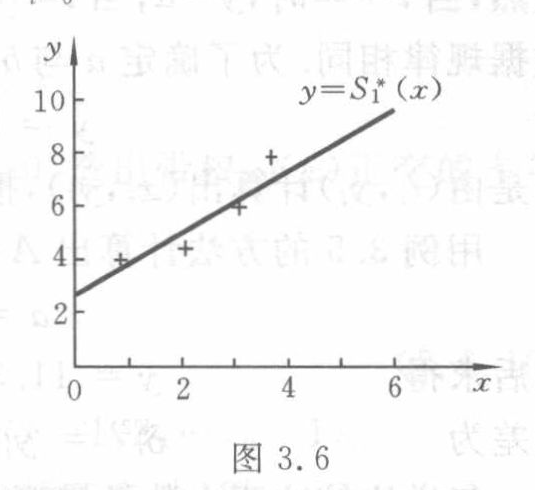
\includegraphics[width=0.85\linewidth,height=\textheight,keepaspectratio,alt={图 3.6（原图裁切）}]{verified/assets/ch03b/figure-3-6.png}

\textbf{图 3.6}（原图裁切）。图中以十字标记数据点，并画出拟合直线 \(y=S_1^*(x)\)。图中文字与符号：\(x,y,0\)；横轴标值 \(2,4,6\)，纵轴标值 \(2,4,6,8,10\)；曲线标签 \(y=S_1^*(x)\)。

\textbf{例 3.6} 在某化学反应过程中，根据实验所得生成物的质量分数与时间的关系如表 3.4 所示，求质量分数 \(y\) 与时间 \(t\) 的拟合曲线 \(y=F(t)\)。

\textbf{表 3.4}

{\def\LTcaptype{none} % do not increment counter
\begin{longtable}[]{@{}
  >{\raggedright\arraybackslash}p{(\linewidth - 32\tabcolsep) * \real{0.0448}}
  >{\raggedleft\arraybackslash}p{(\linewidth - 32\tabcolsep) * \real{0.0597}}
  >{\raggedleft\arraybackslash}p{(\linewidth - 32\tabcolsep) * \real{0.0597}}
  >{\raggedleft\arraybackslash}p{(\linewidth - 32\tabcolsep) * \real{0.0597}}
  >{\raggedleft\arraybackslash}p{(\linewidth - 32\tabcolsep) * \real{0.0597}}
  >{\raggedleft\arraybackslash}p{(\linewidth - 32\tabcolsep) * \real{0.0597}}
  >{\raggedleft\arraybackslash}p{(\linewidth - 32\tabcolsep) * \real{0.0597}}
  >{\raggedleft\arraybackslash}p{(\linewidth - 32\tabcolsep) * \real{0.0597}}
  >{\raggedleft\arraybackslash}p{(\linewidth - 32\tabcolsep) * \real{0.0597}}
  >{\raggedleft\arraybackslash}p{(\linewidth - 32\tabcolsep) * \real{0.0597}}
  >{\raggedleft\arraybackslash}p{(\linewidth - 32\tabcolsep) * \real{0.0597}}
  >{\raggedleft\arraybackslash}p{(\linewidth - 32\tabcolsep) * \real{0.0597}}
  >{\raggedleft\arraybackslash}p{(\linewidth - 32\tabcolsep) * \real{0.0597}}
  >{\raggedleft\arraybackslash}p{(\linewidth - 32\tabcolsep) * \real{0.0597}}
  >{\raggedleft\arraybackslash}p{(\linewidth - 32\tabcolsep) * \real{0.0597}}
  >{\raggedleft\arraybackslash}p{(\linewidth - 32\tabcolsep) * \real{0.0597}}
  >{\raggedleft\arraybackslash}p{(\linewidth - 32\tabcolsep) * \real{0.0597}}@{}}
\toprule\noalign{}
\begin{minipage}[b]{\linewidth}\raggedright
\(t/\mathrm{min}\)
\end{minipage} & \begin{minipage}[b]{\linewidth}\raggedleft
1
\end{minipage} & \begin{minipage}[b]{\linewidth}\raggedleft
2
\end{minipage} & \begin{minipage}[b]{\linewidth}\raggedleft
3
\end{minipage} & \begin{minipage}[b]{\linewidth}\raggedleft
4
\end{minipage} & \begin{minipage}[b]{\linewidth}\raggedleft
5
\end{minipage} & \begin{minipage}[b]{\linewidth}\raggedleft
6
\end{minipage} & \begin{minipage}[b]{\linewidth}\raggedleft
7
\end{minipage} & \begin{minipage}[b]{\linewidth}\raggedleft
8
\end{minipage} & \begin{minipage}[b]{\linewidth}\raggedleft
9
\end{minipage} & \begin{minipage}[b]{\linewidth}\raggedleft
10
\end{minipage} & \begin{minipage}[b]{\linewidth}\raggedleft
11
\end{minipage} & \begin{minipage}[b]{\linewidth}\raggedleft
12
\end{minipage} & \begin{minipage}[b]{\linewidth}\raggedleft
13
\end{minipage} & \begin{minipage}[b]{\linewidth}\raggedleft
14
\end{minipage} & \begin{minipage}[b]{\linewidth}\raggedleft
15
\end{minipage} & \begin{minipage}[b]{\linewidth}\raggedleft
16
\end{minipage} \\
\midrule\noalign{}
\endhead
\bottomrule\noalign{}
\endlastfoot
\(y/\times10^{-3}\) & 4.00 & 6.40 & 8.00 & 8.80 & 9.22 & 9.50 & 9.70 & 9.86 & 10.00 & 10.20 & 10.32 & 10.42 & 10.50 & 10.55 & 10.58 & 10.60 \\
\end{longtable}
}

\textbf{解} 将所给数据标在坐标纸上，如图 3.7 所示。可以看到，质量分数开始时增加较快，后来逐渐减慢，到一定时间就基本稳定在一个水平上，即当 \(t\to\infty\) 时，\(y\) 趋于某

\begin{quote}
校注（agent 补充）：最小二乘不等式右端的 \(\omega(x_i)\) 后原书印有上标星号，原式已保留。该星号在权函数定义中没有定义，疑为多余印字；与式 (3.6.3) 的一致写法应为 \(\omega(x_i)[S(x_i)-f(x_i)]^2\)。见 \href{verified/assets/ch03b/p080-minimum-inequality.png}{原式放大裁切}。
\end{quote}

\clearpage

原书 PDF 页 81；印刷页码 68。

\href{source-images/pdf-081.jpeg}{查看原页}

个数，故 \(y=F(t)\) 有一水平渐近线。另外，\(t=0\) 时，反应未开始，质量分数为零。根据这些特点，可设想 \(y=F(t)\) 是双曲线型 \(1/y=a+b/t\)，即 \(y=t/(at+b)\)。它与给定数据的规律大致符合。

为了确定 \(a,b\)，令 \(\bar y=1/y,x=1/t\)，于是可用 \(x\) 的线性函数 \(S_1(x)=a+bx\) 拟合数据 \((x_i,\bar y_i)\)（\(i=1,2,\cdots,16\)），\(x_i,\bar y_i\) 由原始数据 \((t_i,y_i)\) 根据变换计算出来。与例 3.5 方法相同，解方程组

\[
\begin{cases}
16a+3.38073b=1.8372\times10^3,\\
3.38073a+1.58435b=0.52886\times10^3,
\end{cases}
\]

得

\[
a=80.6621,\quad b=161.6822.
\]

从而得到

\[
y=t/(80.6621t+161.6822)=F^{(1)}(t),
\]

其误差为

\[
\delta_i^{(1)}=y_i-F^{(1)}(t_i)\quad(i=1,2,\cdots,16).
\]

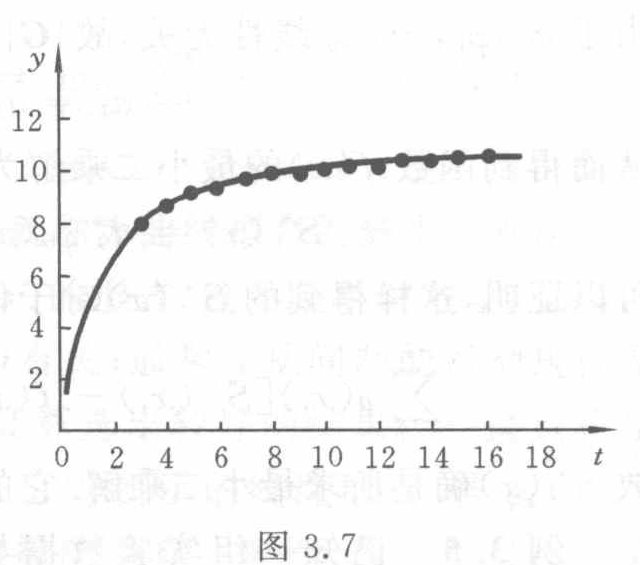
\includegraphics[width=0.85\linewidth,height=\textheight,keepaspectratio,alt={图 3.7（原图裁切）}]{verified/assets/ch03b/figure-3-7.png}

\textbf{图 3.7}（原图裁切）。实验数据点及逐渐趋于水平的拟合曲线。图中文字与符号：纵轴 \(y\)，横轴 \(t\)，原点 \(0\)；横轴标值 \(2,4,6,8,10,12,14,16,18\)，纵轴标值 \(2,4,6,8,10,12\)。

由图 3.7，符合给定数据的函数还可选为指数形式。此时可令拟合曲线形如

\[
y=a\mathrm e^{b/t}.
\]

显然，当 \(t\to\infty\) 时，\(y\to a\)；当 \(t\to0\) 时，若 \(b<0\)，则 \(y\to0\)，且 \(t\) 增加时 \(y\) 增加。这些与给出数据规律相同。为了确定 \(a\) 与 \(b\)，对上式两端取对数，得 \(\ln y=\ln a+b/t\)。令

\[
\hat y=\ln y,\quad A=\ln a,\quad x=1/t,
\]

于是由 \((t_i,y_i)\) 计算出 \((x_i,\hat y_i)\)，拟合数据 \((x_i,y_i)\) 的曲线仍为 \(S_1(x)=A+bx\)。

用例 3.5 的方法计算出 \(A=-4.48072,b=-1.0567\)，从而

\[
a=\mathrm e^A=11.3253\times10^{-3},
\]

最后求得

\[
y=11.3253\times10^{-3}\mathrm e^{-1.0567t}=F^{(2)}(t),
\]

误差为

\[
\delta_i^{(2)}=y_i-F^{(2)}(t_i)\quad(i=1,2,\cdots,16).
\]

怎样比较这两个数学模型的好坏呢？只要分别计算各点误差，从中挑选误差较小的模型即可。本例经过计算可得

\[
\|\boldsymbol\delta^{(1)}\|_\infty=\max_i|\delta_i^{(1)}|=0.568\times10^{-3},
\]

\[
\|\boldsymbol\delta^{(2)}\|_\infty=\max_i|\delta_i^{(2)}|=0.277\times10^{-3},
\]

而均方误差为

\[
\|\boldsymbol\delta^{(1)}\|_2=\sqrt{\sum_{i=1}^m(\delta_i^{(1)})^2}=1.19\times10^{-3},
\]

\[
\|\boldsymbol\delta^{(2)}\|_2=\sqrt{\sum_{i=1}^m(\delta_i^{(2)})^2}=0.34\times10^{-3},
\]

\begin{quote}
校注（agent 补充）：本页最终 \(F^{(2)}(t)\) 的原书指数明确印为 \(-1.0567t\)，已保留。由上文设定 \(y=a\mathrm e^{b/t}\) 及 \(b=-1.0567\)，相容表达式应为 \(\mathrm e^{-1.0567/t}\)；前者在 \(t\to\infty\) 时趋于零，与本页给出的模型性质和数据不相容，属疑似原书漏印除号。见 \href{verified/assets/ch03b/p081-exponential-fit.png}{原式放大裁切}。上文``拟合数据 \((x_i,y_i)\)''亦按原印保留，其语境对应的是变换后的 \((x_i,\hat y_i)\)。
\end{quote}

\clearpage

原书 PDF 页 82；印刷页码 69。

\href{source-images/pdf-082.jpeg}{查看原页}

由此可知，\(\|\boldsymbol\delta^{(2)}\|_2\) 及 \(\|\boldsymbol\delta^{(2)}\|_\infty\) 都比较小，所以用 \(y=F^{(2)}(t)\) 作拟合曲线比较好。

从本例看到，拟合曲线的数学模型并不是一开始就能选得好的，往往要通过分析确定若干模型后，再经过实际计算，才能选到较好的模型。本例的指数模型就比双曲线模型好。

现在很多计算机配有自动选择数学模型的程序，其方法与本例相同。程序中因变量与自变量变换的函数类型较多，通过计算比较误差找到拟合得较好的曲线，最后输出曲线图形及数学表达式。

\subsubsection{3.6.2 用正交函数作最小二乘拟合}\label{ch03b-ux7528ux6b63ux4ea4ux51fdux6570ux4f5cux6700ux5c0fux4e8cux4e58ux62dfux5408}

用最小二乘法得到的法方程组 (3.6.6)，其系数矩阵 \(G\) 是病态的，但如果 \(\varphi_0(x),\varphi_1(x),\cdots,\varphi_n(x)\) 是关于点集 \(\{x_i\}\)（\(i=0,1,\cdots,m\)）带权 \(\omega(x_i)\)（\(i=0,1,\cdots,m\)）正交的函数族，即

\[
(\varphi_j,\varphi_k)=\sum_{i=0}^m\omega(x_i)\varphi_j(x_i)\varphi_k(x_i)=\begin{cases}0,&j\ne k,\\ A_k>0,&j=k,\end{cases}\tag{3.6.8}
\]

则方程组 (3.6.6) 的解为

\[
a_k^*=\frac{(f,\varphi_k)}{(\varphi_k,\varphi_k)}=\frac{\displaystyle\sum_{i=0}^m\omega(x_i)f(x_i)\varphi_k(x_i)}{\displaystyle\sum_{i=0}^m\omega(x_i)\varphi_k^2(x_i)}\quad(k=0,1,\cdots,n),\tag{3.6.9}
\]

且平方误差为

\[
\|\delta\|_2^2=\|f\|_2^2-\sum_{k=0}^n A_k(a_k^*)^2.
\]

现在根据给定节点 \(x_0,x_1,\cdots,x_m\) 及权函数 \(\omega(x)>0\)，造出带权 \(\omega(x)\) 正交的多项式 \(\{P_n(x)\}\)。注意 \(n\leqslant m\)，用递推公式表示 \(P_k(x)\)，即

\[
\begin{cases}
P_0(x)=1,\\
P_1(x)=(x-\alpha_1)P_0(x),\\
P_{k+1}(x)=(x-\alpha_{k+1})P_k(x)-\beta_kP_{k-1}(x)\quad(k=1,2,\cdots,n-1).
\end{cases}\tag{3.6.10}
\]

这里 \(P_k(x)\) 是首项系数为 \(1\) 的 \(k\) 次多项式。根据 \(P_k(x)\) 的正交性，得

\[
\left\{\begin{aligned}
a_{k+1}&=\frac{\displaystyle\sum_{i=0}^m\omega(x_i)x_iP_k^2(x_i)}{\displaystyle\sum_{i=0}^m\omega(x_i)P_k^2(x_i)}=\frac{(xP_k(x),P_k(x))}{(P_k(x),P_k(x))}=\frac{(xP_k,P_k)}{(P_k,P_k)},\\
\beta_k&=\frac{\displaystyle\sum_{i=0}^m\omega(x_i)P_k^2(x_i)}{\displaystyle\sum_{i=0}^m\omega(x_i)P_{k-1}^2(x_i)}=\frac{(P_k,P_k)}{(P_{k-1},P_{k-1})}
\end{aligned}\right.\quad(k=0,1,\cdots,n-1).\tag{3.6.11}
\]

\begin{quote}
校注（agent 补充）：式 (3.6.11) 第一行原书印为拉丁字母 \(a_{k+1}\)，式 (3.6.10) 则为希腊字母 \(\alpha_{k+1}\)，已分别保留。该式末的共同范围原书为 \(k=0,1,\cdots,n-1\)；若直接用于第二行 \(\beta_k\)，\(k=0\) 会涉及未定义的 \(P_{-1}\)。依式 (3.6.10)，实际递推使用的是 \(\beta_1,\ldots,\beta_{n-1}\)。见 \href{verified/assets/ch03b/p082-recursion-coefficients.png}{原式裁切}。
\end{quote}

\clearpage

原书 PDF 页 83；印刷页码 70。

\href{source-images/pdf-083.jpeg}{查看原页}

下面用归纳法证明这样给出的 \(\{P_k(x)\}\) 是正交的。由式 (3.6.10) 第二式及式 (3.6.11) 中 \(a_1\) 的表达式，有

\[
\begin{aligned}
(P_l,P_1)&=(P_0,xP_0)-\alpha_1(P_0,P_0)\\
&=(P_0,xP_0)-\frac{(xP_0,P_0)}{(P_0,P_0)}(P_0,P_0)=0.
\end{aligned}
\]

现假定 \((P_1,P_s)=0\)（\(l\ne s\)）对于 \(s=0,1,\cdots,l-1\) 及 \(l=0,1,\cdots,k\)（\(k<n\)）均成立，要证 \((P_{k+1},P_s)=0\) 对于 \(s=0,1,\cdots,k\) 均成立。由式 (3.6.10)，有

\[
\begin{aligned}
(P_{k+1},P_s)&=((x-\alpha_{k+1})P_k,P_s)-\beta_k(P_{k-1},P_s)\\
&=(xP_k,P_s)-\alpha_{k+1}(P_k,P_s)-\beta_k(P_{k-1},P_s),
\end{aligned}\tag{3.6.12}
\]

由归纳法假定，当 \(0\leqslant s\leqslant k-2\) 时

\[
(P_k,P_s)=0,\quad(P_{k-1},P_s)=0.
\]

另外，\(xP_s(x)\) 是首项系数为 \(1\) 的 \(s+1\) 次多项式，它可用 \(P_0,P_1,\cdots,P_{s+1}\) 的线性组合表示，而 \(s+1\leqslant k-1\)，故由归纳法假定又有

\[
(xP_k,P_s)\equiv(P_k,xP_s)=0,
\]

于是由式 (3.6.12)，当 \(s\leqslant k-2\) 时，\((P_{k+1},P_s)=0\)。

再看

\[
(P_{k+1},P_{k-1})=(xP_k,P_{k-1})-\alpha_{k+1}(P_k,P_{k-1})-\beta_k(P_{k-1},P_{k-1}),\tag{3.6.13}
\]

由假定有

\[
(P_k,P_{k-1})=0,
\]

\[
(xP_k,P_{k-1})=(P_k,xP_{k-1})=\left(P_k,P_k+\sum_{j=0}^{k-1}C_jP_j\right)=(P_k,P_k).
\]

利用式 (3.6.11) 的 \(\beta_k\) 表达式及以上结果，得

\[
(P_{k+1},P_{k-1})=(xP_k,P_{k-1})-\beta_k(P_{k-1},P_{k-1})=(P_k,P_k)-(P_k,P_k)=0.
\]

最后，由式 (3.6.11) 有

\[
\begin{aligned}
(P_{k+1},P_k)&=(xP_k,P_k)-\alpha_{k+1}(P_k,P_k)-\beta_k(P_k,P_{k-1})\\
&=(xP_k,P_k)-\frac{(xP_k,P_k)}{(P_k,P_k)}(P_k,P_k)=0.
\end{aligned}
\]

至此已证明了由式 (3.6.10) 及式 (3.6.11) 确定的多项式，\(\{P_k(x)\}\)（\(k=0,1,\cdots,n;n\leqslant m\)）组成一个关于点集 \(\{x_i\}\) 的正交系。

用正交多项式 \(\{P_k(x)\}\) 的线性组合作最小二乘曲线拟合，只要在根据式 (3.6.10) 及式 (3.6.11) 逐步求 \(P_k(x)\) 的同时，相应计算出系数

\[
a_k=\frac{(f,P_k)}{(P_k,P_k)}=\frac{\displaystyle\sum_{i=0}^m\omega(x_i)f(x_i)P_k(x_i)}{\displaystyle\sum_{i=0}^m\omega(x_i)P_k^2(x_i)}\quad(k=0,1,\cdots,n),
\]

并逐步把 \(\alpha_k^*P_k(x)\) 累加到 \(F(x)\) 中去，最后就可得到所求的拟合曲线

\[
y=F(x)=\alpha_0^*P_0(x)+\alpha_1^*P_1(x)+\cdots+\alpha_n^*P_n(x),
\]

\begin{quote}
校注（agent 补充）：本页第一式左端原扫描为 \((P_l,P_1)\)（第一下标为字母 \(l\)），依右端计算应对应 \((P_0,P_1)\)。下一段归纳假设原印为 \((P_1,P_s)=0\)，括号内条件却为 \(l\ne s\)，疑应为 \((P_l,P_s)=0\)。均忠实保留并见 \href{verified/assets/ch03b/p083-induction-start.png}{原文裁切}。页尾系数公式用 \(a_k\)，其后累加与拟合曲线改用 \(\alpha_k^*\)，也按原印保留；此处应是同一组拟合系数的记号不一致，不应与递推系数 \(\alpha_k\) 混用。见 \href{verified/assets/ch03b/p083-fit-coefficients.png}{原文裁切}。
\end{quote}

\clearpage

原书 PDF 页 84；印刷页码 71。

\href{source-images/pdf-084.jpeg}{查看原页}

这里 \(n\) 可事先给定或在计算过程中根据误差确定。

用这种方法编程序不用解方程组，只用递推公式，并且当逼近次数增加一次时，只要把程序中循环数加 \(1\)，其余不用改变。这是目前用多项式作曲线拟合最好的计算方法，有通用的语言程序供用户使用。

\subsubsection{3.6.3 多元最小二乘拟合}\label{ch03b-ux591aux5143ux6700ux5c0fux4e8cux4e58ux62dfux5408}

上面介绍的最小二乘法的有关概念与方法可推广到多元函数，例如，已知多元函数

\[
y=f(x_1,x_2,\cdots,x_l)
\]

的一组测量数据 \((x_{1i},x_{2i},\cdots,x_{li},y_i)\)（\(i=1,2,\cdots,m\)），以及一组权系数 \(\omega_i>0\)（\(i=1,2,\cdots,m\)），要求函数

\[
S_n(x_1,x_2,\cdots,x_l)=\sum_{k=1}^na_k\varphi_k(x_1,x_2,\cdots,x_l),\quad n\leqslant m,
\]

使得

\[
F(a_0,a_1,\cdots,a_n)=\sum_{i=1}^m\omega_i[y_i-S_n(x_{1i},x_{2i},\cdots,x_{li})]^2
\]

最小，这与式 (3.6.4) 的极值问题完全一样，系数 \(a_0,a_2,\cdots,a_n\) 同样满足法方程组 (3.6.6)，只是这里

\[
(\varphi_k,\varphi_j)=\sum_{i=1}^m\omega_i\varphi_k(x_{1i},x_{2i},\cdots,x_{li})\varphi_i(x_{1i},x_{2i},\cdots,x_{li}).
\]

求解法方程组 (3.6.6) 就可得到 \(a_k\)（\(k=0,1,\cdots,n\)），从而得到 \(S_n(x_1,x_2,\cdots,x_l)\)。称 \(S_n(x_1,x_2,\cdots,x_l)\) 为函数 \(f(x_1,x_2,\cdots,x_l)\) 的最小二乘拟合。

\subsection{3.7 Fourier 逼近与快速 Fourier 变换}\label{ch03b-fourier-ux903cux8fd1ux4e0eux5febux901f-fourier-ux53d8ux6362}

当 \(f(x)\) 是周期函数时，显然用三角多项式比用代数多项式逼近更合适，本节主要讨论用三角多项式作最小平方逼近及快速 Fourier 变换（Fast Fourier Transform），简称 FFT 算法。

\subsubsection{3.7.1 最佳平方三角逼近与三角插值}\label{ch03b-ux6700ux4f73ux5e73ux65b9ux4e09ux89d2ux903cux8fd1ux4e0eux4e09ux89d2ux63d2ux503c}

设 \(f(x)\) 是以 \(2\pi\) 为周期的平方可积函数，用三角多项式

\[
S_n(x)=\frac12a_0+a_1\cos x+b_1\sin x+\cdots+a_n\cos nx+b_n\sin nx\tag{3.7.1}
\]

作最佳平方逼近函数。由于三角函数族 \(1,\cos x,\sin x,\cdots,\cos kx,\sin kx,\cdots\) 在 \([0,2\pi]\) 上是正交函数族，于是 \(f(x)\) 在 \([0,2\pi]\) 上的最小平方三角逼近多项式 \(S_n(x)\) 的系数是

\begin{quote}
校注（agent 补充）：3.6.3 原书的 \(S_n\) 求和从 \(k=1\) 开始，但后续使用 \(F(a_0,a_1,\ldots,a_n)\) 和 \(a_k\;(k=0,\ldots,n)\)；段中系数列表印为 \(a_0,a_2,\ldots,a_n\)；内积公式右端第二因子的原印下标为 \(i\)，而左端为 \(j\)，相容写法应使用 \(\varphi_j\)。这些原书记号不一致均已保留，见 \href{verified/assets/ch03b/p084-multivariate-formulas.png}{原文裁切}。
\end{quote}

\clearpage

原书 PDF 页 85；印刷页码 72。

\href{source-images/pdf-085.jpeg}{查看原页}

\[
\begin{cases}
a_k=\dfrac1\pi\displaystyle\int_0^{2\pi}f(x)\cos kx\,\mathrm dx\quad(k=0,1,\cdots,n),\\[4pt]
b_k=\dfrac1\pi\displaystyle\int_0^{2\pi}f(x)\sin kx\,\mathrm dx\quad(k=1,2,\cdots,n),
\end{cases}\tag{3.7.2}
\]

\(a_k,b_k\) 称为 Fourier 系数，函数 \(f(x)\) 按 Fourier 系数展开得到的级数

\[
\frac12a_0+\sum_{k=1}^{\infty}(a_k\cos kx+b_k\sin kx)\tag{3.7.3}
\]

就称为 Fourier 级数，只要 \(f'(x)\) 在 \([0,2\pi]\) 上分段连续，则级数 (3.7.3) 一致收敛到 \(f(x)\)。

当 \(f(x)\) 只在给定的离散点集 \(\left\{x_j=\dfrac{2\pi}{N}j,\ j=0,1,\cdots,N-1\right\}\) 上已知时，则可类似得到在离散点集上的正交性与相应的离散 Fourier 系数。为方便起见，下面只给出奇数个点的情形。令

\[
x_j=\frac{2\pi j}{2m+1}\quad(j=0,1,\cdots,2m),
\]

可以证明，对于任何 \(0\leqslant k,l\leqslant m\)，成立

\[
\left\{\begin{aligned}
\sum_{j=0}^{2m}\sin lx_j\sin kx_j&=\begin{cases}
0,&l\ne k,\ l=k=0,\\
\dfrac{2m+1}{2},&l=k\ne0,
\end{cases}\\[4pt]
\sum_{j=0}^{2m}\cos lx_j\cos kx_j&=\begin{cases}
0,&l\ne k,\\
\dfrac{2m+1}{2},&l=k\ne0,\\
2m+1,&l=k=0,
\end{cases}\\[4pt]
\sum_{j=0}^{2m}\cos lx_j\sin kx_j&=0,\quad0\leqslant k,j\leqslant m.
\end{aligned}\right.
\]

这就表明，函数族 \(\{1,\cos x,\sin x,\cdots,\cos mx,\sin mx\}\) 在点集 \(\left\{x_j=\dfrac{2\pi j}{2m+1}\right\}\) 上正交。若令 \(f_j=f(x_j)\)（\(j=0,1,\cdots,2m\)），则 \(f(x)\) 的最小二乘三角逼近为

\[
S_n(x)=\frac12a_0+\sum_{k=1}^n(a_k\cos kx+b_k\sin kx),\quad n<m,
\]

其中

\[
\begin{cases}
a_k=\dfrac2{2m+1}\displaystyle\sum_{j=0}^{2m}f_j\cos\dfrac{2\pi jk}{2m+1}\quad(k=0,1,\cdots,n),\\[4pt]
b_k=\dfrac2{2m+1}\displaystyle\sum_{j=0}^{2m}f_j\sin\dfrac{2\pi jk}{2m+1}\quad(k=1,\cdots,n).
\end{cases}\tag{3.7.4}
\]

当 \(n=m\) 时，可证明 \(S_m(x_j)=f_j\)（\(j=0,1,\cdots,2m\)），于是

\[
S_m(x)=\frac12a_0+\sum_{k=1}^m(a_k\cos kx+b_k\sin kx)
\]

\begin{quote}
校注（agent 补充）：离散正交性公式的最后一行，原书条件为 \(0\leqslant k,j\leqslant m\)，已保留。这里 \(j\) 是求和指标，函数频率为 \(k,l\)；与该组公式前的条件一致时应写 \(0\leqslant k,l\leqslant m\)。
\end{quote}

\clearpage

原书 PDF 页 86；印刷页码 73。

\href{source-images/pdf-086.jpeg}{查看原页}

就是三角插值多项式，系数仍由式 (3.7.4) 表示。

更一般情形，假定 \(f(x)\) 是以 \(2\pi\) 为周期的复函数，给定在 \(N\) 个等分点 \(x_j=\dfrac{2\pi}{N}j\)（\(j=0,1,\cdots,N-1\)）上的值 \(f_j=f\left(\dfrac{2\pi}{N}j\right)\)，由于

\[
\mathrm e^{\mathrm ijx}=\cos(jx)+\mathrm i\sin(jx)\quad(j=0,1,\cdots,N-1;\ \mathrm i=\sqrt{-1}),
\]

函数族 \(\{1,\mathrm e^{\mathrm ix},\cdots,\mathrm e^{\mathrm i(N-1)x}\}\) 在区间 \([0,2\pi]\) 上是正交的。将函数 \(\mathrm e^{\mathrm ijx}\) 在等距点集 \(x_k=\dfrac{2\pi}{N}k\)（\(k=0,1,\cdots,N-1\)）上的值 \(\mathrm e^{\mathrm ijx_k}\) 组成的向量记作

\[
\boldsymbol\varphi_j=\left(1,\mathrm e^{\mathrm ij\frac{2\pi}{N}},\cdots,\mathrm e^{\mathrm ij\frac{2\pi}{N}(N-1)}\right)^{\mathrm T}.
\]

当 \(j=0,1,\cdots,N-1\) 时，\(N\) 个复向量 \(\boldsymbol\varphi_0,\boldsymbol\varphi_1,\cdots,\boldsymbol\varphi_{N-1}\) 具有下面所定义的正交性：

\[
(\boldsymbol\varphi_l,\boldsymbol\varphi_s)=\sum_{k=0}^{N-1}\mathrm e^{\mathrm il\frac{2\pi}{N}k}\mathrm e^{-\mathrm is\frac{2\pi}{N}k}=\sum_{k=0}^{N-1}\mathrm e^{\mathrm i(l-s)\frac{2\pi}{N}k}=\begin{cases}0,&l\ne s,\\N,&l=s.\end{cases}\tag{3.7.5}
\]

事实上，令 \(r=\mathrm e^{\mathrm i(l-s)\frac{2\pi}{N}}\)，若 \(0\leqslant l,s\leqslant N-1\)，则有

\[
0\leqslant l\leqslant N-1,\quad-(N-1)\leqslant-s\leqslant0,
\]

于是

\[
-(N-1)\leqslant l-s\leqslant N-1,\quad-1<-\frac{N-1}{N}\leqslant\frac{l-s}{N}\leqslant\frac{N-1}{N}<1.
\]

若 \(l-s\ne0\)，则 \(r\ne1\)，从而 \(r^N=\mathrm e^{\mathrm i(l-s)2\pi}=1\)，于是

\[
(\boldsymbol\varphi_l,\boldsymbol\varphi_s)=\sum_{k=0}^{N-1}r^k=\frac{1-r^N}{1-r}=0.
\]

若 \(l=s\)，则 \(r=1\)，于是 \((\boldsymbol\varphi_s,\boldsymbol\varphi_s)=\sum_{k=0}^{N-1}r^k=N\)。这就证明了式 (3.7.5) 成立，即 \(\boldsymbol\varphi_0,\boldsymbol\varphi_1,\cdots,\boldsymbol\varphi_{N-1}\) 是正交的。

因此，\(f(x)\) 在 \(N\) 个点 \(\left\{x_j=\dfrac{2\pi}{N}j,\ j=0,1,\cdots,N-1\right\}\) 上的最小二乘 Fourier 逼近为

\[
S(x)=\sum_{k=0}^{n-1}C_k\mathrm e^{\mathrm ikx},\quad n\leqslant N,\tag{3.7.6}
\]

其中

\[
C_k=\frac1N\sum_{j=0}^{N-1}f_j\mathrm e^{-\mathrm ikj\frac{2\pi}{N}}\quad(k=0,1,\cdots,N-1).\tag{3.7.7}
\]

在式 (3.7.6) 中，若 \(n=N\)，则 \(S(x)\) 为 \(f(x)\) 在点 \(x_j\)（\(j=0,1,\cdots,N-1\)）上的插值函数，即 \(S(x_j)=f(x_j)\)，于是由式 (3.7.6) 得

\[
f_j=\sum_{k=0}^{N-1}C_k\mathrm e^{\mathrm ik\frac{2\pi}{N}j}\quad(j=0,1,\cdots,N-1).\tag{3.7.8}
\]

式 (3.7.7) 表示了由 \(\{f_j\}\) 求 \(\{C_k\}\) 的过程，称为 \(f(x)\) 的离散 Fourier 变换，简称

\clearpage

原书 PDF 页 87；印刷页码 74。

\href{source-images/pdf-087.jpeg}{查看原页}

DFT；而式 (3.7.8) 是由 \(\{C_k\}\) 求 \(\{f_j\}\) 的过程，称为反变换。它们是使用计算机进行 Fourier 分析的主要方法，在数字信号处理、全息技术、光谱和声谱分析等很多领域都有广泛应用。

\subsubsection{3.7.2 快速 Fourier 变换}\label{ch03b-ux5febux901f-fourier-ux53d8ux6362}

不论是按式 (3.7.7) 由 \(\{f_k\}\) 求 \(\{C_j\}\)，按式 (3.7.8) 由 \(\{C_j\}\) 求 \(\{f_k\}\)，还是由式 (3.7.4) 计算 Fourier 逼近系数 \(a_k,b_k\)，都可归结为计算

\[
C_j=\sum_{k=0}^{N-1}x_kw^{kj}\quad(j=0,1,\cdots,N-1),\tag{3.7.9}
\]

其中 \(w=\exp(-\mathrm i2\pi/N)\)（正变换）或 \(w=\exp(\mathrm i2\pi/N)\)（反变换）；\(\{x_k\}\)（\(k=0,1,\cdots,N-1\)）是已知复数序列。如直接用式 (3.7.9) 计算 \(C_j\)，需要 \(N\) 次复数乘法和 \(N\) 次复数加法（称为 \(N\) 个操作），计算全部 \(C_j\) 共要 \(N^2\) 个操作。当 \(N\) 较大且处理数据很多时，就是用高速的电子计算机，很多实际问题仍然无法计算，直到 20 世纪 60 年代中期产生了快速 Fourier 变换，即 FFT 算法，大大提高了运算速度，才使 Fourier 变换得以广泛应用。FFT 算法的思想就是尽量减少乘法次数，例如，计算 \(ab+ac=a(b+c)\)，用左端计算时做两次乘法，用右端计算时只做一次乘法。用式 (3.7.9) 计算全部 \(C_j\)，表面看要做 \(N^2\) 次乘法，实际上，在所有 \(\exp(\mathrm i2\pi kj/N),\ j,k=0,1,\cdots,N-1\) 中，只有 \(N\) 个不同的值 \(w^0,w^1,\cdots,w^{N-1}\)，特别当 \(N=2^p\) 时，只有 \(N/2\) 个不同的值。因此，可把同一个 \(w^r\) 对应的 \(x_k\) 相加后再乘 \(w^r\)，这样就能大量减少乘法次数。为了具体推导 FFT 算法，先给出定义：

设正整数 \(m\) 除以 \(N\) 后得商 \(q\) 及余数 \(r\)，则 \(m=qN+r\)，\(r\) 称为 \(m\) 的 \(N\) 同余数。由于 \(w=\exp(\mathrm i2\pi/N),w^N=\mathrm e^{\mathrm i2\pi}=1\)，故有 \(w^m=(w^N)^qw^r=w^r\)。

因此计算 \(w^m\) 时可用 \(w\) 的 \(N\) 同余数 \(r\) 代替 \(m\)，从而推出 FFT 算法。下面以 \(N=2^3\) 为例说明 FFT 的计算方法。由于 \(0\leqslant k,j\leqslant N-1=2^3-1=7\)，则式 (3.7.9) 的和是

\[
C_j=\sum_{k=0}^7x_kw^{jk}\quad(j=0,1,\cdots,7).\tag{3.7.10}
\]

将 \(k,j\) 用二进制表示为

\[
k=k_2 2^2+k_1 2+k_0 2^0=(k_2k_1k_0),
\]

\[
j=j_2 2^2+j_1 2^1+j_0 2^0=(j_2j_1j_0),
\]

其中 \(k_r,j_r\)（\(r=0,1,2\)）只能取 \(0\) 或 \(1\)，例如，\(6=2^2+2^1+0\times2^0=(110)\)。根据 \(k,j\) 表示法，有 \(C_j=C(j_2j_1j_0),x_k=x(k_2k_1k_0)\)。式 (3.7.10) 可表示为

\[
\begin{aligned}
C(j_2j_1j_0)&=\sum_{k_0=0}^1\sum_{k_1=0}^1\sum_{k_2=0}^1x(k_2k_1k_0)w^{(k_2k_1k_0)(j_2 2^2+j_1 2^1+j_0 2^0)}\\
&=\sum_{k_0=0}^1\left\{\sum_{k_1=0}^1\left[\sum_{k_2=0}^1x(k_2k_1k_0)w^{j_0(k_2k_1k_0)}\right]w^{j_1(k_1k_0 0)}\right\}\left(w^{j_2(k_0 00)}\right).
\end{aligned}\tag{3.7.11}
\]

\begin{quote}
校注（agent 补充）：原书``特别当 \(N=2^p\) 时，只有 \(N/2\) 个不同的值''已保留。对原文列出的全部 \(\exp(\mathrm i2\pi kj/N)\) 而言，取 \(j=1\) 已有 \(N\) 个不同值；若利用 \(w^{r+N/2}=-w^r\)，才可用 \(N/2\) 个值及符号表示它们。因此该处``不同的值''疑漏了``除符号外''一类限定。原书``可用 \(w\) 的 \(N\) 同余数 \(r\) 代替 \(m\)''也按原文保留，根据前段定义，此处应是指数 \(m\) 的余数。
\end{quote}

\clearpage

原书 PDF 页 88；印刷页码 75。

\href{source-images/pdf-088.jpeg}{查看原页}

若引入记号

\[
\begin{cases}
A_0(k_2k_1k_0)=x(k_2k_1k_0),\\[4pt]
A_1(k_1k_0j_0)=\displaystyle\sum_{k_2=0}^1A_0(k_2k_1k_0)w^{j_0(k_2k_1k_0)},\\[4pt]
A_2(k_0j_1j_0)=\displaystyle\sum_{k_1=0}^1A_1(k_1k_0j_0)w^{j_1(k_1k_0 0)},\\[4pt]
A_3(j_2j_1j_0)=\displaystyle\sum_{k_0=0}^1A_2(k_0j_1j_0)w^{j_2(k_0 00)},
\end{cases}\tag{3.7.12}
\]

则式 (3.7.11) 变成

\[
C(j_2j_1j_0)=A_3(j_2j_1j_0).
\]

它说明利用 \(N\) 同余数可把计算 \(C_j\) 分为 \(p\) 步，用式 (3.7.12) 计算，每计算一个 \(A_q\) 只用 \(2\) 次复数乘法，计算一个 \(C_j\) 用 \(2p\) 次复数乘法，计算全部 \(C_j\) 共用 \(2pN\) 次复数乘法。若注意 \(w^{j_0 2^{p-1}}=w^{j_0N/2}=(-1)^j\)，式 (3.7.12) 还可进一步简化为

\[
\begin{aligned}
A_1(k_1k_0j_0)&=\sum_{k_2=0}^1A_0(k_2k_1k_0)w^{j_0(k_2k_1k_0)}\\
&=A_0(0k_1k_0)w^{j_0(0k_1k_0)}+A_0(1k_1k_0)w^{j_0 2^2}w^{j_0(0k_1k_0)}\\
&=[A_0(0k_1k_0)+(-1)^{j_0}A_0(1k_1k_0)]w^{j_0(0k_1k_0)},
\end{aligned}
\]

\[
A_1(k_1k_0 0)=A_0(0k_1k_0)+A_0(1k_1k_0),
\]

\[
A_1(k_1k_0 1)=[A_0(0k_1k_0)-A_0(1k_1k_0)]w^{(0k_1k_0)}.
\]

将表达式中的二进制表示还原为十进制表示：\(k=(0k_1k_0)=k_1 2^1+k_0 2^0\)，即 \(k=0,1,2,3\)，得

\[
\begin{cases}
A_1(2k)=A_0(k)+A_0(k+2^2),\\
A_1(2k+1)=[A_0(k)-A_0(k+2^2)]w^k
\end{cases}\quad(k=0,1,2,3).\tag{3.7.13}
\]

同样，式 (3.7.12) 中的 \(A_2\) 可简化为

\[
A_2(k_0j_1j_0)=[A_1(0k_0j_0)+(-1)^{j_1}A_1(1k_0j_0)]w^{j_1(0k_0 0)},
\]

即

\[
A_2(k_0 0j_0)=A_1(0k_0j_0)+A_1(1k_0j_0),
\]

\[
A_2(k_0 1j_0)=[A_1(0k_0j_0)-A_1(1k_0j_0)]w^{(0k_0 0)}.
\]

将表达式中的二进制表示还原为十进制表示，得

\[
\begin{cases}
A_2(k2^2+j)=A_1(2k+j)+A_1(2k+j+2^2),\quad k=0,1,\\
A_2(k2^2+j+2)=[A_1(2k+j)-A_1(2k+j+2^2)]w^{2k},\quad j=0,1.
\end{cases}\tag{3.7.14}
\]

同样，式 (3.7.12) 中 \(A_3\) 可简化为

\[
A_3(j_2j_1j_0)=A_2(0j_1j_0)+(-1)^{j_2}A_2(1j_1j_0),
\]

即

\[
A_3(0j_1j_0)=A_2(0j_1j_0)+A_2(1j_1j_0),
\]

\[
A_3(1j_1j_0)=A_2(0j_1j_0)-A_2(1j_1j_0).
\]

\clearpage

原书 PDF 页 89；印刷页码 76。

\href{source-images/pdf-089.jpeg}{查看原页}

将表达式中的二进制表示还原为十进制表示，得

\[
\begin{cases}
A_3(j)=A_2(j)+A_2(j+2^2),\\
A_3(j+2^2)=A_2(j)-A_2(j+2^2)
\end{cases}\quad(j=0,1,2,3).\tag{3.7.15}
\]

根据式 (3.7.13)、式 (3.7.14)、式 (3.7.15)，由 \(A_0(k)=x(k)=x_k\)（\(k=0,1,\cdots,7\)）逐次计算到 \(A_3(j)=C_j\)（\(j=0,1,\cdots,7\)），结果如表 3.5 所示。

\textbf{表 3.5}

{\def\LTcaptype{none} % do not increment counter
\begin{longtable}[]{@{}
  >{\raggedright\arraybackslash}p{(\linewidth - 16\tabcolsep) * \real{0.1111}}
  >{\raggedright\arraybackslash}p{(\linewidth - 16\tabcolsep) * \real{0.1111}}
  >{\raggedright\arraybackslash}p{(\linewidth - 16\tabcolsep) * \real{0.1111}}
  >{\raggedright\arraybackslash}p{(\linewidth - 16\tabcolsep) * \real{0.1111}}
  >{\raggedright\arraybackslash}p{(\linewidth - 16\tabcolsep) * \real{0.1111}}
  >{\raggedright\arraybackslash}p{(\linewidth - 16\tabcolsep) * \real{0.1111}}
  >{\raggedright\arraybackslash}p{(\linewidth - 16\tabcolsep) * \real{0.1111}}
  >{\raggedright\arraybackslash}p{(\linewidth - 16\tabcolsep) * \real{0.1111}}
  >{\raggedright\arraybackslash}p{(\linewidth - 16\tabcolsep) * \real{0.1111}}@{}}
\toprule\noalign{}
\begin{minipage}[b]{\linewidth}\raggedright
单元码号
\end{minipage} & \begin{minipage}[b]{\linewidth}\raggedright
(0) 000
\end{minipage} & \begin{minipage}[b]{\linewidth}\raggedright
(1) 001
\end{minipage} & \begin{minipage}[b]{\linewidth}\raggedright
(2) 010
\end{minipage} & \begin{minipage}[b]{\linewidth}\raggedright
(3) 011
\end{minipage} & \begin{minipage}[b]{\linewidth}\raggedright
(4) 100
\end{minipage} & \begin{minipage}[b]{\linewidth}\raggedright
(5) 101
\end{minipage} & \begin{minipage}[b]{\linewidth}\raggedright
(6) 110
\end{minipage} & \begin{minipage}[b]{\linewidth}\raggedright
(7) 111
\end{minipage} \\
\midrule\noalign{}
\endhead
\bottomrule\noalign{}
\endlastfoot
& & & & & \(w^0=1\) & \(w^1\) & \(w^2\) & \(w^3\) \\
\(x_k=A_0(k)\) & \(A_0(0)\) & \(A_0(1)\) & \(A_0(2)\) & \(A_0(3)\) & \(A_0(4)\) & \(A_0(5)\) & \(A_0(6)\) & \(A_0(7)\) \\
\(A_1\) & \(A_0(0)+A_0(4)\) & \([A_0(0)-A_0(4)]w^0\) & \(A_0(1)+A_0(5)\) & \([A_0(1)-A_0(5)]w^1\) & \(A_0(2)+A_0(6)\) & \([A_0(2)-A_0(6)]w^2\) & \(A_0(3)+A_0(7)\) & \([A_0(3)-A_0(7)]w^3\) \\
\(A_2\) & \(A_1(0)+A_1(4)\) & \(A_1(0)+A_1(5)\) & \([A_1(0)-A_1(4)]w^0\) & \([A_1(1)-A_1(5)]w^0\) & \(A_1(2)+A_1(6)\) & \(A_1(3)+A_1(7)\) & \([A_1(2)-A_1(6)]w^2\) & \([A_1(3)-A_1(7)]w^2\) \\
\(C_i=A_3(j)\) & \((0)+(4)\) & \((1)+(5)\) & \((2)+(6)\) & \((3)+(7)\) & \((0)-(4)\) & \((1)-(5)\) & \((2)-(6)\) & \((3)-(7)\) \\
\end{longtable}
}

\href{verified/assets/ch03b/table-3-5-source.png}{表 3.5 原图裁切}。

上面推导的 \(N=2^3\) 的计算公式可类似地推广到 \(N=2^p\) 的情形。根据式 (3.7.13)、式 (3.7.14)、式 (3.7.15)，一般情况的 FFT 计算公式如下：

\[
\left\{\begin{aligned}
A_q(k2^q+j)&=A_{q-1}(k2^{q-1}+j)+A_{q-1}(k2^{q-1}+j+2^{p-1}),\\
A_q(k2^q+j+2^{q-1})&=[A_{q-1}(k2^{q-1}+j)-A_{q-1}(k2^{q-1}+j+2^{p-1})]w^{k2^{q-1}},
\end{aligned}\right.\tag{3.7.16}
\]

其中 \(q=1,2,\cdots,p;\ k=0,1,\cdots,2^{p-q}-1;\ j=0,1,\cdots,2^{q-1}-1\)。\(A_q\) 括号内的数代表它的位置，在计算机中代表存放数的地址。一组 \(A_q\) 占用 \(N\) 个复数单元，计算时需给出两组单元，从 \(A_0(m)\)（\(m=0,1,\cdots,N-1\)）出发，\(q\) 由 \(1\) 到 \(p\) 算到 \(A_p(j)=C_j\)（\(j=0,1,\cdots,N-1\)），即为所求。计算过程中只要按地址号存放 \(A_q\)，最后得到的 \(A_p(j)\) 就是所求离散频谱的次序（注意，目前一些计算机程序计算结果地址是逆序排列，还要增加倒地址的一步才是这里介绍的结果）。这个计算公式不仅具有不倒地址的优点，而且计算只有两重循环，外循环 \(q\) 由 \(1\) 计算到 \(p\)，内循环 \(k\) 由 \(0\) 计算到 \(2^{p-q}-1\)，\(j\) 由 \(0\) 计算到 \(2^{q-1}-1\)，更重要的是整个计算过程计算量小。由公式可看到，算一个 \(A_q\) 共做 \(2^{p-q}2^{q/1}=N/2\) 次复数乘法；而最后一步计算 \(A_p\) 时，由于 \(w^{k2^{p-1}}=(w^{N/2})^k=(-1)^k=(-1)^0=1\)（注意，\(q=p\) 时 \(2^{p-q}-1=0\)，故 \(k=0\)），因此，总共要算 \((p-1)N/2\) 次复数乘法，它比直接用式 (3.7.9) 计算需 \(N^2\) 次乘法快得多，计算量之比是 \(N:(p-1)/2\)。当 \(N=2^{10}\) 时二者之比是 \(1024:4.5\approx230:1\)。它比一般 FFT 的计算量 \(pN\) 次乘法

\begin{quote}
校注（agent 补充）：表 3.5 的 \(A_2\) 行、单元 (1) 原书为 \(A_1(0)+A_1(5)\)，按式 (3.7.14) 代入 \(k=0,j=1\) 应为 \(A_1(1)+A_1(5)\)；表末行标签原书为 \(C_i=A_3(j)\)，与正文 \(C_j\) 的记号不一致。两处均按原印保留。运算量段落原印为 \(2^{p-q}2^{q/1}=N/2\)，放大可辨指数中为斜杠，依前文循环次数应为 \(2^{p-q}2^{q-1}=N/2\)。见 \href{verified/assets/ch03b/p089-operation-count.png}{运算量原式裁切}。
\end{quote}

\clearpage

原书 PDF 页 90；印刷页码 77。

\href{source-images/pdf-090.jpeg}{查看原页}

也快一倍。式 (3.7.16) 的计算公式称为改进的 FFT 算法，下面给出这一算法的程序步骤：

\textbf{步 1} 给出数组 \(A_1(N),A_2(N)\) 及 \(w(N/2)\)。

\textbf{步 2} 将已知的记录复数数组 \(\{x_k\}\) 输入到单元 \(A_1(k)\)（\(k\) 从 \(0\) 到 \(N-1\)）中。

\textbf{步 3} 计算 \(w^m=\exp\left(-\mathrm i\dfrac{2\pi}{N}m\right)\) 或 \(w^m=\exp\left(\mathrm i\dfrac{2\pi}{N}m\right)\)，存放在单元 \(w(m)\)（\(m\) 从 \(0\) 到 \((N/2)-1\)）中。

\textbf{步 4} \(q\) 循环从 \(1\) 到 \(p\)，若 \(q\) 为奇数做步 5，否则做步 6。

\textbf{步 5} \(k\) 循环从 \(0\) 到 \(2^{p-q}-1\)，\(j\) 循环从 \(0\) 到 \(2^{q-1}-1\)，计算

\[
A_2(k2^q+j)=A_1(k2^{q-1}+j)+A_1(k2^{q-1}+j+2^{p-1}),
\]

\[
A_2(k2^q+j+2^{q-1})=[A_1(k2^{q-1}+j)-A_1(k2^{q-1}+j+2^{q-1})]w(k2^{q-1}),
\]

转步 7。

\textbf{步 6} \(k\) 循环从 \(0\) 到 \(2^{p-q}-1\)，\(j\) 循环从 \(0\) 到 \(2^{q-1}\)，计算

\[
A_1(k2^q+j)=A_2(k2^{q-1}+j)+A_2(k2^{q-1}+j+2^{p-1}),
\]

\[
A_1(k2^q+j+2^{q-1})=[A_2(k2^{q-1}+j)-A_2(k2^{q-1}+j+2^{q-1})]w(k2^{q-1}),
\]

\(k,j\) 循环结束，做下一步。

\textbf{步 7} 若 \(q=p\) 转步 8，否则 \(q+1\to q\) 转步 4。

\textbf{步 8} \(q\) 循环结束，若 \(p=\text{偶数}\)，将 \(A_1(j)\to A_2(j)\)，则 \(C_j=A_2(j)\)（\(j=0,1,\cdots,N-1\)）即为所求。

\subsection{小结}\label{ch03b-ux5c0fux7ed3}

函数逼近是数学中一个很重要的课题，本章只介绍了函数逼近最基本的概念及常用的正交多项式，并从函数计算观点介绍了用多项式逼近连续函数的主要方法。这些都是计算数学的基础，需要详细了解的读者可参看文献 {[}4{]}。本章对函数逼近与计算的另一重要课题------有理逼近没有涉及，这方面内容可参看文献 {[}5{]}。

本章介绍的曲线拟合的最小二乘法和离散 Fourier 变换都可从最佳平方逼近得到，它们在实际中都有广泛的应用，本章着重介绍了在计算机上有效和节省时间的算法，而不要求理论上的详细讨论。特别是 FFT 算法，不但应用中意义重大，而且也是计算数学中节省运算次数的一个典范。本章介绍的改进 FFT 算法比目前使用的 FFT 算法计算次数又减少了，程序也较简单，这一算法的推导与应用可参看文献 {[}6{]}。

\subsection{习题}\label{ch03b-ux4e60ux9898}

\textbf{1.} （1）利用区间变换推出区间为 \([a,b]\) 的 Bernstein 多项式。

\begin{quote}
校注（agent 补充）：步 5、步 6 的差式中，第二个读取地址的偏移量原书均印为 \(2^{q-1}\)，与式 (3.7.16) 的 \(2^{p-1}\) 不一致；正文保留原式。步 6 的 \(j\) 循环上界原印为 \(2^{q-1}\)，相较式 (3.7.16) 与步 5 少了``\(-1\)''。按该上界执行会多计算一个 \(j\)，在 \(q=p\) 时也会越出 \(N\) 个数组单元范围。见 \href{verified/assets/ch03b/p090-fft-steps.png}{原程序步骤裁切}。
\end{quote}

\clearpage

原书 PDF 页 91；印刷页码 78。

\href{source-images/pdf-091.jpeg}{查看原页}

（2）对 \(f(x)=\sin x\) 在 \([0,\pi/2]\) 上求一次和三次 Bernstein 多项式，画出图形，并与相应的 Taylor 级数部分和误差作比较。

\textbf{2.} 求证：

（1）当 \(m\leqslant f(x)\leqslant M\) 时，\(m\leqslant B_n(f,x)\leqslant M\)；（2）当 \(f(x)=x\) 时，\(B_n(f,x)=x\)。

\textbf{3.} 在次数不超过 \(6\) 的多项式中，求 \(f(x)=\sin4x\) 在 \([0,2\pi]\) 上的最佳一致逼近多项式。

\textbf{4.} 假设 \(f(x)\) 在 \([a,b]\) 上连续，求 \(f(x)\) 的零次最佳一致逼近多项式。

\textbf{5.} 选取常数 \(a\)，使 \(\max\limits_{0\leqslant x\leqslant1}|x^3-ax|\) 达到极小，又问这个解是否唯一。

\textbf{6.} 求 \(f(x)=\sin x\) 在 \([0,\pi/2]\) 上的最佳一次逼近多项式，并估计误差。

\textbf{7.} 求 \(f(x)=\mathrm e^x\) 在 \([0,1]\) 上的最佳一次逼近多项式。

\textbf{8.} 如何选取 \(r\)，使 \(p(x)=x^2+r\) 在 \([-1,1]\) 上与零偏差最小？\(r\) 是否唯一？

\textbf{9.} 设 \(f(x)=x^4+3x^3-1\)，在 \([0,1]\) 上求三次最佳逼近多项式。

\textbf{10.} 令 \(T_n(x)=T_n(2x-1),x\in[0,1]\)，求 \(T_0^*(x),T_1^*(x),T_2^*(x),T_3^*(x)\)。

\textbf{11.} 试证 \(\{T_n^*(x)\}\) 是在 \([0,1]\) 上带权 \(\rho=\dfrac1{\sqrt{x-x^2}}\) 的正交多项式。

\textbf{12.} \(f(x)\) 是 \([-a,a]\) 上的连续奇（偶）函数，证明：不管 \(n\) 是奇数或偶数，\(f(x)\) 的最佳逼近多项式 \(F_n^*(x)\in H_n\) 也是奇（偶）函数。

\textbf{13.} 求 \(a,b\)，使 \(\displaystyle\int_0^{\frac\pi2}[ax+b-\sin x]^2\,\mathrm dx\) 为最小，并与题 1 及题 6 的一次逼近多项式误差作比较。

\textbf{14.} \(f(x),g(x)\in C^1[a,b]\)，定义

（1）\((f,g)=\displaystyle\int_a^b f'(x)g'(x)\,\mathrm dx\)，

（2）\((f,g)=\displaystyle\int_a^b f'(x)g'(x)\,\mathrm dx+f(a)g(a)\)，

它们是否构成内积？

\textbf{15.} 用 Schwarz 不等式 (3.4.5) 估计 \(\displaystyle\int_0^1\frac{x^6}{1+x}\,\mathrm dx\) 的上界，并用积分中值定理估计同一积分的上、下界，并比较其结果。

\textbf{16.} 选择 \(a\)，使积分 \(\displaystyle\int_{-1}^1(x-ax^2)^2\,\mathrm dx\)，\(\displaystyle\int_{-1}^1|x-ax^2|\,\mathrm dx\) 取得最小值。

\textbf{17.} 设 \(\varphi_1=\operatorname{span}\{1,x\},\varphi_2=\operatorname{span}\{x^{100},x^{101}\}\)，分别在 \(\varphi_1,\varphi_2\) 上求一元素，使其为 \(x^2\in C[0,1]\) 的最佳平方逼近，并比较其结果。

\textbf{18.} \(f(x)=|x|\) 在 \([-1,1]\) 上，求在 \(\varphi_1=\operatorname{span}\{1,x^2,x^4\}\) 上的最佳平方逼近。

\textbf{19.} \(u_n(x)=\dfrac{\sin[(n+1)\arccos x]}{\sqrt{1-x^2}}\) 是第二类 Chebyshev 多项式，证明它有递推关系

\[
u_{n+1}(x)=2xu_n(x)-u_{n-1}(x).
\]

\textbf{20.} 将 \(f(x)=\sin\dfrac12x\) 在 \([-1,1]\) 上按 Legendre 多项式及 Chebyshev 多项式展开，求三次最佳平方逼近多项式并画出误差图形，再计算均方误差。

\textbf{21.} 把 \(f(x)=\arccos x\) 在 \([-1,1]\) 上展开成 Chebyshev 级数。

\textbf{22.} 用最小二乘法求一个形如 \(y=a+bx^2\) 的经验公式，使它与表 3.6 所示数据相拟合，并求均方误差。

\begin{quote}
校注（agent 补充）：题 10 的定义左端原书为 \(T_n(x)\)，后面要求的是 \(T_0^*,T_1^*,T_2^*,T_3^*\)，且题 11 使用 \(T_n^*\)；定义左端疑漏星号，应为 \(T_n^*(x)=T_n(2x-1)\)。题 15 的 Schwarz 不等式引用原书印为 (3.4.5)，本章 Schwarz 不等式的编号为 (3.3.5)，疑为交叉引用误印。两处均保留原文，见 \href{verified/assets/ch03b/p091-exercise-10.png}{题10原图裁切}、\href{verified/assets/ch03b/p091-exercise-15.png}{题15原图裁切}。
\end{quote}

\clearpage

原书 PDF 页 92；印刷页码 79。

\href{source-images/pdf-092.jpeg}{查看原页}

\textbf{表 3.6}

{\def\LTcaptype{none} % do not increment counter
\begin{longtable}[]{@{}lrrrrr@{}}
\toprule\noalign{}
\(x_i\) & 19 & 25 & 31 & 38 & 44 \\
\midrule\noalign{}
\endhead
\bottomrule\noalign{}
\endlastfoot
\(y_i\) & 19.0 & 32.3 & 49.0 & 73.3 & 97.8 \\
\end{longtable}
}

\textbf{23.} 观察物体的直线运动，得出时间 \(t\) 与距离 \(s\) 的关系如表 3.7 所示，求运动方程。

\textbf{表 3.7}

{\def\LTcaptype{none} % do not increment counter
\begin{longtable}[]{@{}lrrrrrr@{}}
\toprule\noalign{}
\(t/\mathrm s\) & 0 & 0.9 & 1.9 & 3.0 & 3.9 & 5.0 \\
\midrule\noalign{}
\endhead
\bottomrule\noalign{}
\endlastfoot
\(s/\mathrm m\) & 0 & 10 & 30 & 50 & 80 & 110 \\
\end{longtable}
}

\textbf{24.} 在某化学反应里，根据实验所得分解物的质量分数 \(y\) 与时间 \(t\) 的关系如表 3.8 所示，用最小二乘拟合求 \(y=F(t)\)。

\textbf{表 3.8}

{\def\LTcaptype{none} % do not increment counter
\begin{longtable}[]{@{}lrrrrrr@{}}
\toprule\noalign{}
\(t/\mathrm{min}\) & 0 & 5 & 10 & 15 & 20 & 25 \\
\midrule\noalign{}
\endhead
\bottomrule\noalign{}
\endlastfoot
\(y/\times10^{-4}\) & 0 & 1.27 & 2.16 & 2.86 & 3.44 & 3.87 \\
\(t/\mathrm{min}\) & 30 & 35 & 40 & 45 & 50 & 55 \\
\(y/\times10^{-4}\) & 4.15 & 4.37 & 4.51 & 4.58 & 4.62 & 4.64 \\
\end{longtable}
}

\textbf{25.} 编出用正交多项式作最小二乘拟合的程序框图。

\textbf{26.} 编出改进 FFT 算法的程序框图。

\textbf{27.} 已知 \(\{x_k\}=(4,3,2,1,0,1,2,3)\)，用改进 FFT 算法求 \(\{x_k\}\) 离散频谱 \(\{C_k\}\)（\(k=0,1,\cdots,7\)）。

